\section{State observer}

Implementing an advanced control mechanism such as \textit{linear quadratic controller}, \textit{full state feedback} or in our case, \textit{model predictive controller}, requires a knowledge of all system states values. This is a different situation then in the case of previously used PID controller, when only the controlled state needs to be known. There are some situations and corresponding systems, where the knowledge of all states values is relatively easy to obtain, respectively it might be already measured for another reason. For instance space, aerials or another vehicles, where the typical states are position and its derivatives. But in the case where not all states can be measured or we do not want to measure them, the state observer needs to be implemented. The state observer is a dynamical system which is simulated concurrently with the controlled system. It has the same number of inputs and it is controlled by the same actions as the real system. The order of the observer is the same as the order of the system. Its states are supposed to be observable and should correspond to the real system's states.

\subsection{Open-loop observer}

Let us have an LTI system that needs to be observed (assuming $\textbf{C} = \textbf{I}$, $\textbf{D} = \mathbf{0}$ i.e. the output consists directly of all states and there is no direct transfer from the input to the output). The uncertainty in the model or some external disturbance is covered by the vector $\textbf{w}$ which is unknown and usually called a \emph{process noise}.

\begin{equation}
\textbf{x}_{[t+1]} = \textbf{A}\textbf{x}_{[t]} + \textbf{B}\textbf{u}_{[t]} + \textbf{w}_{[t]}
\end{equation}

The open-loop observer can be constructed by setting up following system where $\textbf{\^x}$ denotes a vector of estimated state values. When $\textbf{w}$ has non zero-mean $\textbf{\^x}$ is going to drift from $\textbf{x}$ since the process noise is integrated over time.

\begin{equation}
\textbf{\^x}_{[t+1]} = \textbf{A}\textbf{\^x}_{[t]} + \textbf{B}\textbf{u}_{[t]}
\label{eq:openloop_observer}
\end{equation}

Three distinct situations can be expected to happen during the execution:

\begin{itemize}
\item Estimated states track well corresponding system states. The system was identified perfectly and there is no need for feedback control in this situation.
\item Estimated states track well system sates, but there is some drift during the time frame of the experiment. The feedback loop is required to provide zero-offset observation.
\item States estimated by the observer are completely out of scope of real system states which may suggest that the observer's model is wrong.
\end{itemize}

Open-loop estimations in the chapter \ref{cap:system_identification} indicate that out model is in our case satisfactory but the open-loop estimator would not probably lead to precise control results.

\subsection{Closed-loop observer}

The open-loop observer can be basically corrected by closing a feedback loop around the system as follows.

\begin{equation}
\textbf{\^x}_{[t+1]} = \textbf{A}\textbf{\^x}_{[t]} + \textbf{B}\textbf{u}_{[t]} - \textbf{L}\left(\textbf{x}_{[t]} - \textbf{\^x}_{[t]}\right)
\label{eq:closed_loop_observer}
\end{equation}

There are methods of finding $\textbf{L}$ such that poles of the observer are desirably placed\footnote{Assuming the system can be converted to the \textit{controlled canonical form}}. One can utilize that placing poles of a state feedback is a dual problem for placing poles of the observer. Practically one can tune a state feedback controller using matrices $\textbf{A}^T, \textbf{B}^T$ to get $\textbf{L}^T$ for the observer.

\subsection{Kalman filter}

For the purpose of this thesis, the Kalman filter was implemented to estimate all states of the helicopter and to filter the measured data from sensors. The Kalman filter is a closed-loop iterative estimator. A hypothesis about estimated states takes form of a normal distribution with mean vector $\hat{\textbf{x}}$ and covariance matrix $\hat{\boldsymbol{\Sigma}}$. It presumes a model in a following form

\begin{equation}
\textbf{x}_{[t+1]} = \textbf{A}\textbf{x}_{[t]} + \textbf{B}\textbf{u}_{[t]} + \textbf{w}_{[t]}
\label{eq:kalman_model}
\end{equation}

where \textbf{w} is the process noise which is supposed to be drawn from normal distribution $\mathcal{N}(\textbf{0}, \textbf{R})$. Furthermore there is a sensor model

\begin{equation}
\textbf{z}_{[t]} = \textbf{H}\textbf{x}_{[t]} + \textbf{v}_{[t]}
\end{equation}

where $\textbf{z}$ is a measurement vector, \textbf{H} is a matrix that maps the state vector to the measurement and $\textbf{v}$ is the measurement noise which is supposed to be drawn from $\mathcal{N}(\textbf{0}, \textbf{Q})$. A real measurement is modeled using the sensor model by adding a sample of the measurement noise to all states and transforming it by \textbf{H} to a measurement vector. The filter holds a state vector $\textbf{\^x}$ and its covariance matrix $\hat{\boldsymbol{\Sigma}}$ between iterations.

\begin{table}[h]
\centering
\begin{tabular}{ccccc}
\hline
& vector & covariance & mapping to \textbf{\^x} & mapping to \textbf{z}\\
\hline
estimated states & \textbf{\^x} & $\hat{\boldsymbol{\Sigma}}$ & \textbf{I} & \textbf{P}\\
measurement & \textbf{z} & \textbf{Q} & \textbf{H} & \textbf{I}\\
model (process) & \textbf{x} & \textbf{R} & & \\
\hline
\end{tabular}
\caption{Overview of vectors and matrices used in Kalman filter.}
\label{tab:matrices_in_kalman}
\end{table}

\subsubsection{Prediction phase}

There are two phases of the Kalman filter algorithm. Figure \ref{fig:kalman_diagram} shows the block diagram for better clarity. The first one is the \textit{prediction phase} (\ref{eq:kalman_prediction}) which can be easily compared to the open-loop observer (\ref{eq:openloop_observer}). Here the new state vector is estimated using the model (\ref{eq:kalman_model}), previous state $\textbf{\^x}_{[t-1]}$ and the input $\textbf{u}_{[t-1]}$. Its covariance $\hat{\boldsymbol{\Sigma}}_{[t]}$ is modified using the model and the process noise covariance $\textbf{R}$.

\begin{equation}
\begin{split}
\hat{\textbf{x}}_{[t]} &\leftarrow \textbf{A}\hat{\textbf{x}}_{[t-1]} + \textbf{B}\textbf{u}_{[t-1]} \\
\hat{\boldsymbol{\Sigma}}_{[t]} &\leftarrow \textbf{A}\hat{\boldsymbol{\Sigma}}_{[t-1]}\textbf{A}^{T} + \textbf{R}
\end{split}
\label{eq:kalman_prediction}
\end{equation}    

\subsubsection{Correction phase}
The second phase is the \textit{correction phase} (\ref{eq:kalman_correction}) where the state vector is updated using a measurement $\textbf{z}_{[t]}$. The covariance $\hat{\boldsymbol{\Sigma}}_{[t]}$ is modified again but this time using the noise measurement covariance \textbf{Q}. Following assignment statements denote the correction phase of the Kalman filter

\begin{equation}
\begin{split}
\textbf{K}_{[t]} &\leftarrow \hat{\boldsymbol{\Sigma}}_{[t]}\textbf{P}^{T}\left(\textbf{P}\hat{\boldsymbol{\Sigma}}_{[t]}\textbf{P}^{T} + \textbf{Q}\right)^{-1} \\
\hat{\textbf{x}}_{[t]} &\leftarrow \hat{\textbf{x}}_{[t]} + \textbf{K}_{[t]}\left(\textbf{z}_{[t]} - \textbf{P}\hat{\textbf{x}}_{[t]}\right) \\
\hat{\boldsymbol{\Sigma}}_{[t]} &\leftarrow \left(\mathbf{I} - \textbf{K}_{[t]}\textbf{P}\right)\hat{\boldsymbol{\Sigma}}_{[t]}
\end{split}
\label{eq:kalman_correction}
\end{equation}

where $\textbf{K}_t$ is the Kalman gain, $\mathbf{I}$ is the identity matrix, \textbf{P} is the matrix that maps estimated states to the measurement. The first part consists of computing a Kalman gain $\textbf{K}_t$. It has a direct correspondence to the matrix \textbf{L} in (\ref{eq:closed_loop_observer}) thus it determines the feedback effect in the observer. The gain can be fine tuned by carefully setting \textbf{R} and \textbf{Q}. The \textbf{Q} can be found by observing the noise parameters of measurements. That means the process noise is left for us to set. The table \ref{tab:matrices_in_kalman} denotes the important vectors and matrices that are used in the filter. Practically there is a trade-off between trusting fully to the model and trusting fully to sensors. When setting \textbf{R} the filtered values have to be observed and the Kalman filter should be set basically by tuning the ratio between elements of \textbf{R} and \textbf{Q}. The desired outcome usually is to eliminate the measurement noise while still preserving the zero-offset tracking (with sufficient transient response) of all estimated states.

\begin{figure}
\centering
\begin{tikzpicture}[->,>=stealth']

 % Position of PREDICTION 
 % Use previously defined 'state' as layout (see above)
 % use tabular for content to get columns/rows
 % parbox to limit width of the listing
 \node[state] (PREDICTION) 
 {
 \begin{tabular}{c}
  	\textbf{Prediction} \\
  	\begin{tabular}{rcl}
	$\hat{\textbf{x}}_{[t]}$ & $\leftarrow$ & $\textbf{A}\hat{\textbf{x}}_{[t-1]} + \textbf{B}\textbf{u}_{[t-1]}$ \\
	$\hat{\boldsymbol{\Sigma}}_{[t]}$ & $\leftarrow$ & $\textbf{A}\hat{\boldsymbol{\Sigma}}_{[t-1]}\textbf{A}^{T} + \textbf{R}$
 	\end{tabular}
 \end{tabular}
 };
  
 % State: CORRECTION with different content
 \node[state,    	% layout (defined above)
  below of=PREDICTION, 	% Position is to the right of PREDICTION
  node distance=4cm, 	% distance to PREDICTION
  anchor=center] (CORRECTION) 	% posistion relative to the center of the 'box'
 {%
 \begin{tabular}{c}
  	\textbf{Correction} \\
  	\begin{tabular}{rcl}
		$\textbf{K}_{[t]}$ & $\leftarrow$ & $\hat{\boldsymbol{\Sigma}}_{[t]}\textbf{P}^{T}\left(\textbf{P}\hat{\boldsymbol{\Sigma}}_{[t]}\textbf{P}^{T} + \textbf{Q}\right)^{-1}$ \\
		$\hat{\textbf{x}}_{[t]}$ & $\leftarrow$ & $\hat{\textbf{x}}_{[t]} + \textbf{K}_{[t]}\left(\textbf{z}_{[t]} - \textbf{P}\hat{\textbf{x}}_{[t]}\right)$ \\
		$\hat{\boldsymbol{\Sigma}}_{[t]}$ & $\leftarrow$ & $\left(\mathbf{I} - \textbf{K}_{[t]}\textbf{P}\right)\hat{\boldsymbol{\Sigma}}_{[t]}$ \\
 	\end{tabular}
 \end{tabular}
 };
 
 \node[nothing,    	% layout (defined above)
  left of=PREDICTION, 	% Position is to the right of QUERY
  node distance=5cm, 	% distance to QUERY
  anchor=center] (PRED_IN) 	% posistion relative to the center of the 'box'
 {};
 
 \node[nothing,    	% layout (defined above)
  left of=CORRECTION, 	% Position is to the right of QUERY
  node distance=7cm, 	% distance to QUERY
  anchor=center] (CORR_IN) 	% posistion relative to the center of the 'box'
 {};

 % draw the paths and and print some Text below/above the graph
 \path (PREDICTION) 	edge[bend left=30]  node[anchor=west]
 	   {
 		$\hat{\textbf{x}}_{[t]}$, $\hat{\boldsymbol{\Sigma}}_{[t]}$
       } (CORRECTION)
       (CORRECTION) 	edge[bend left=30]  node[anchor=east]
 	   {
 	   	\begin{tabular}{c}
 	   	$\hat{\textbf{x}}_{[t]}$, $\hat{\boldsymbol{\Sigma}}_{[t]}$ \\
 	   	$t \leftarrow t + 1$	
 	   	\end{tabular}
       } (PREDICTION)
       
       (PRED_IN) edge[] node[anchor=south] {\textbf{Input}} node[anchor=north] {\textbf{u}} (PREDICTION)
       
       (CORR_IN) edge[] node[anchor=south] {\textbf{Measurement}} node[anchor=north] {$\textbf{z}, \textbf{Q}, \textbf{P}$} (CORRECTION);

\end{tikzpicture}
\caption{Bock diagram of the Kalman filter}
\label{fig:kalman_diagram}
\end{figure}

\subsection{Summary}

In this chapter the Kalman filter algorithm was presented in order to estimate all system states and filter measured data. Its performance can be shown on subsequence of data (forward movement) used in chapter \ref{cap:attitude_subsystem_identification}. The figure \ref{fig:kalman1} shows the velocity in one of attitude axis of UAV measured by \emph{px4flow} sensor. Among others, it is able to estimate all other states including the position and the acceleration which is essential for further use of model predictive controller. It can be tuned to estimate noisy signal with relatively small delay compared to e.g. exponential filter\footnote{The exponential filter is an easy technique where filtered value is computed as $\textbf{\^x}_{[t]} = \alpha\textbf{\^x}_{[t-1]} + (1-\alpha)\textbf{x}_{[t]}$}. For particular parameters of Kalman filter that are used in the final implementation see chapter \ref{cap:Implementation} where also an extended form of LTI system is presented to provide a disturbance estimation.

\begin{figure}[h]
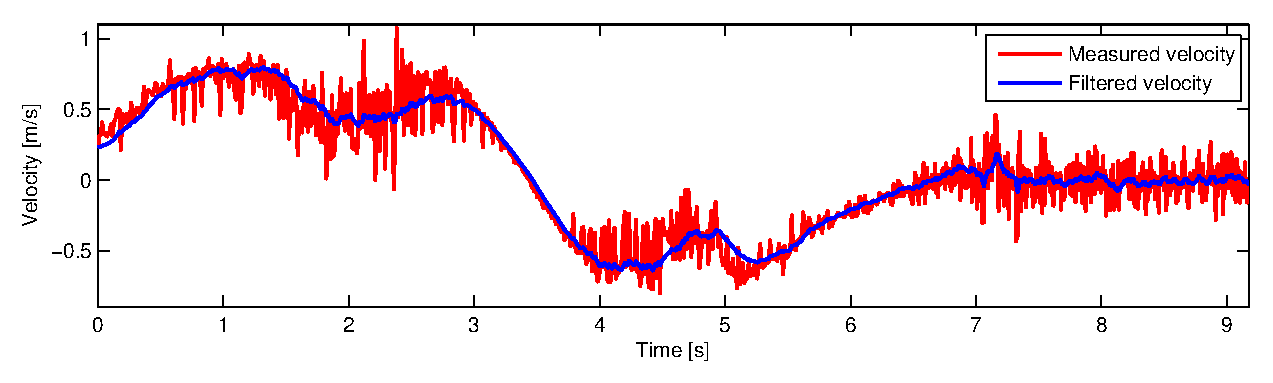
\includegraphics[width=1\textwidth]{fig/kalman1.eps} 
\caption{Kalman filter tracking a noisy singal of UAV's forward speed.}
\label{fig:kalman1}
\end{figure}